%!TEX root = final_report.tex

\section{Results} 

As an indicator of the performance of our model, we report the learning curves
for the label propagation algorithm.  To measure the performance of the model,
we calculate the mean error distance, median error distance, precision and
recall at k curves for different amounts of seed data. 

\begin{table*}[tbp]
\begin{center}
\begin{tabular}{|r|r|r|}
\hline
Percent Training Data & Mean Error Distance & Precision \\
\hline
12.5 & 1870.89 & 37.79 \\
25.0 & 1774.53 & 41.88 \\
50.0 & 1681.29 & 46.69 \\
75.0 & 1625.87 & 49.75 \\
\hline
\end{tabular}
\caption{Mean error and precision for label propagation}
\label{tab:results}
\end{center}
\end{table*}


\begin{figure*}[tbp]
\begin{center}
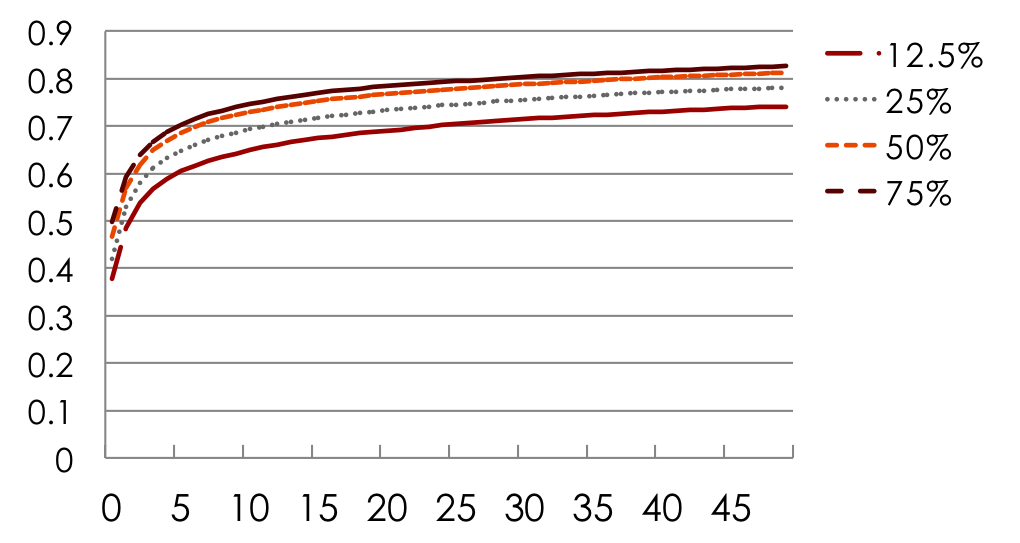
\includegraphics[scale=0.7]{recall_at_k.png}
\caption{Recall at k. The axis is k, the y axis is the fraction of documents for whom the correct label is within the top k predicted labels.}
\label{fig:recall}
\end{center}
\end{figure*}


\begin{table*}[tbp]
\begin{center}
\begin{tabular}{|r|r|r|r|}
\hline
Strategy & Degree & Median & Mean \\
\hline
Kullback - Liebler & 0.1 & 11.8 & 221 \\
Naïve Bayes & 0.1 & 15.5 & 314 \\
Avg. Cell Probability & 0.1 & 24.1 & 1421 \\
Label Propagation & 1 & 0 &  1626 \\
Most Frequent Toponym &  0.5 &  136 & 1927 \\
Cell Prior Maximum & 5 & 2333 & 4309 \\
Random & 0.1 &7259 & 7192 \\
\hline
\end{tabular}
\caption{Comparison of our results with \cite{wing-baldridge:11}. The results reported in \cite{rolleretal:12} are of the same magnitude as KL divergence.}
\label{tab:comparison}
\end{center}
\end{table*}


In our model, the error distance is defined as the distance between the
centers of the predicted and the actual grid cells. \comment{confirm if the
centers of the grid cells are centroids or geometric centers} With this
definition, the mean error distance is the mean of the error distances for all
the test documents. Similarily, the median error distance is the median of
errors for all the documents. \comment{We also show the error curves, which
are a better indicator of system performance.} Precision is defined as the
fraction of test documents for which the model predicts the correct grid cell.
Since our model returns a ranked list of probable grid cells for each
document, \comment{more motivation for why this is a good thing} we also
calculate the recall at k curves for the results. For our experiments, rekall
at k is defined as the fraction of the test documents for which the correct
label is present within to top k grid cells predicted by label propagation.

It should be noted that the error distances are sensitive to the grid size,
since they are calculated as the distance between the centers of predicted and
the actual cells. Because of this, a smaller grid size (up to a point) results
in better mean error distances since the penalty for predicting a neighboring
but only partly correct cell is lower. We leave repeating the experiments with
different grid sizes and adaptive grids as future work.


From the results in Table \ref{tab:results}, it can be observed that the mean
error decreases and the precision increases as we increase the number of
documents with seed labels provided initially. In Table \ref{tab:results}, the
percentages are the percentage of nodes in the geo-tagged graph that
originally have seed labels on them.

The recall at k curves are shown in Figure \ref{fig:recall} and are what one
would expect. The recall increases as we go further down the list of results,
with fairly high (nearly 70\%) recall within the top 10 predicted labels.
There's approximately 10\% difference in recall between label propagation with
12.5\% and 75\% seed documents at all values of k.

We compare the results of our approach with those in \cite{wing-baldridge:11}
and show the results in Table \ref{tab:comparison}. A naive implementation of
label propagation performs much better than the baselines, and comparably to
the average cell probability approach. It should be noted that while the
results are already encouraging, we expect the actual results of a more
rigorous and optimized experimental setup for label propagation to be
significantly better.

We found that increasing the number of iterations in label propagation beyond
a certain number (e.g. 10 iterations for the run with 75\% seed data) does not
significantly change the results, suggesting that the algorithm converges on a
solution relatively quickly.
